\chapter{Konzeptionierung}
\label{ch: Konzeptionierung}

In diesem Kapitel wird die Konzeptionierung der Personenerkennung sowie die der Statemachine für das autonome Logistikfahrzeug erläutert. Wie auch in der vorangegangenen Bachelorarbeit geschah die Anforderungserhebung mit der Methode des \textit{Conceptual design specification technique for the engineering of complex Systems} (CONSENS). Am Institut für Systemtechnik der Hochschule Bochum wird zur systematischen Spezifikation von komplexen Systemen die \textit{CONSENS} Methode geschult. Die Anforderungen an die beschriebenen Teilsysteme wurden im Lastenheft als Anforderungsliste festgehalten. Die Komponenten für die Entwicklung sind im Umfeldmodell und den entsprechenden Wirkstrukturen dargestellt.
	
	
	\section{Anforderungserhebung mit CONSENS}
	\label{sec: Anforderungserhebung}
	
	In Abbildung \ref{fig: consensenv} ist das erweiterte Umfeldmodell des ALFs zu sehen. Das ursprüngliche Umfeldmodell ist in der entsprechenden Bachelorarbeit wiederzufinden \cite{Bachelorarbeit}. Der Aufbau des Entwurfs besteht im Allgemeinen aus hellblauen und gelben Hexagonen, die Wirk- und Umfeldelemente repräsentieren. Der Informationsfluss zwischen den Elementen ist durch gestrichelte Pfeile gekennzeichnet. Das ALF gilt als Kern des Gesamtsystems und ist deswegen im Modell mittig dargestellt. Es interagiert sowohl mit Wirk- als auch mit Umfeldelementen, wie in Abbildung \ref{fig: consensenv} gezeigt. Der Zustandsautomat ist ein Teilsystem, das als Erweiterung des Umfelds gilt. Die von Herrn Dittmann entwickelte Sprachverarbeitung kann sowohl auf dem Rechner des ALFs als auch auf dem integrierten \textit{Raspberry Pi} ausgeführt werden \cite{Dittmann}. Transitionsbedingungen können dementsprechend je nach Anwendungsfall durch beide Hardwarekomponenten intern über das \textit{ROS}-Netzwerk an den EA gesendet werden.       \\
	
	\begin{figure}[H]
	\begin{center}
		\begin{tikzpicture}
			%\node[CONSENSsys] (env3) at (0,0) {ROS system for manual and autonomous driving};
			\node[CONSENSenv] (env1) at (-7,2) {Kinect\\Sensor(1)};
			\node[CONSENSenv] (env2) at (-7,-2) {Kinect\\Sensor(2)};
			\node[CONSENSsys] (sys1) at (-2,0) {ALF};
			\node[CONSENSsys] (sys2) at (-4,4) {Raspberry\\Pi};
			\node[CONSENSenv] (env3) at (0,4) {Bildschirm};
		%	\node[CONSENSenv] (env4) at (3,-2) {Bildschirm};
			\node[CONSENSenv] (env5) at (0,-4) {Fern-\\bedienung};
			\node[CONSENSenv] (env6) at (-4,-4) {Laut-\\sprecher};
			\node[CONSENSenv] (env8) at (3,0) {Antriebs-\\einheit};
			\node[CONSENSenv] (env7) at (-7,0) {Lidar\\Sensor};
			\node[CONSENSenv] (env9) at (3,2) {Zustands-\\automat};
			
			%27 grad von der ebene
			
			\draw[CSarrow,dashed] (env1.0) -| (sys1.153) node[align = left, font = \scriptsize] at (-4.25,2.4) {Audio Signal,\\Bildinformationen};
			\draw[CSarrow,dashed] (env2.0) -| (sys1.207) node[align = left, font = \scriptsize] at (-4.25,-1.6) {Audio Signal,\\Bildinformationen};
			\draw[CSarrow,dashed] (env7) -- (sys1) node[align = left, font = \scriptsize] at (-4.5,0.4) {Umfeld-\\informationen};
			\draw[CSarrow,dashed] (sys2.0) -| node[above,align=center,font=\scriptsize]{Winkel\\Daten}(sys1.90);
			\draw[CSarrow,dashed] (sys1.58) |- (env3.180) node[align = left, font = \scriptsize] at (-1,3) {Visuali-\\sierung};
			\draw[CSarrow,dashed] (sys1.0) -- node[above,font=\scriptsize]{$4$ x Drehzahlen}(env8.180) ;
			\draw[CSarrow,dashed] (env5.90) |- node[right,align=center,font=\scriptsize]{Benutzer-\\eingaben}(sys1.333);
			\draw[CSarrow,dashed] (sys1.270) |- (env6.0) node[align = left, font = \scriptsize] at (-1,-1.7) {Status-\\informationen};	
			\draw[CSarrow,dashed] (sys1.270) |- (env6.0) node[align = left, font = \scriptsize] at (-1,-1.7) {Status-\\informationen};
			\draw[CSarrow,dashed] (sys1.40) |- (env9.153) node[align = left, font = \scriptsize] at (1.25,3) {Transitions-\\bedingung};
			\draw[CSarrow,dashed] (env9.180) -| (sys1.27) node[align = left, font = \scriptsize] at (-0.4,1.5) {Zustand};
			\draw[CSarrow,dashed] (sys1.122) |- (sys2.333) node[align = left, font = \scriptsize] at (-2.9,2.8) {Audio\\Signal};
			\draw[CSarrow,dashed] (sys2.90) |- (3,5)--(env9.90) node[align = left, font = \scriptsize] at (0,5.2) {Transitionsbedingung};
			%% legende
			
			\node (rect) at (3,-2.0) [draw,thick,minimum width=4.5cm,minimum height=1.75cm] {};
			\node [CONSENSlegendenv] [minimum width=3.8mm,minimum height=6.35mm] (env4) at (1.25,-1.4) {};
			\node [CONSENSlegendsys] [minimum width=3.8mm,minimum height=6.35mm] (sys4) at (1.25,-2.0) {};
			\draw[CSarrow,dashed] (1.0,-2.6) -- node[right]{\footnotesize \Umbruch{}}(1.6,-2.6);
			\node [align=left,font=\footnotesize] (txt1) at (3.35,-1.4) {Umfeldelement};
			\node [align=left,font=\footnotesize] (txt2) at (3.35,-2.0) {Wirkelement};
			\node [align=left,font=\footnotesize] (txt3) at (3.35,-2.6) {Information};
			

			\end{tikzpicture}
			\caption{Weiterentwickeltes Umfeldmodell des Systems ALF. Hierbei wurde das System um die Umfeldelemente des Zustandsautomaten und der integrierten Lautsprecher erweitert. \cite{Bachelorarbeit}}
			\label{fig: consensenv}
	\end{center}
\end{figure}	
	
	Die Erweiterung um die Personenerkennung ist in der in Abbildung \ref{fig: consensctrl} gezeigten Wirkstruktur dargestellt. Eine Wirkstruktur repräsentiert den Inhalt eines Wirkelements und dient zum besseren Verständnis komplexer Zusammenhänge. In diesem Fall wird das Wirkelement mit dem Titel ALF aus dem vorangegangenem Umfeldmodell \ref{fig: consensenv} aufgeschlüsselt. Die hier gezeigte Wirkstruktur wurde um die Personenerkennung und die Sprachverarbeitung erweitert. Elemente mit blassen Farben sind für diese Masterarbeit eher unwichtig und werden weiterhin nicht behandelt.\\
	
	Für den Betrieb der Personenerkennung sind die Bildinformationen der integrierten \textit{Kinect}-Kameras notwendig. Als Ausgabe werden zweidimensionale Positionen von erkannten Personen für das Visualisierungsprogramm \textit{RViz} veröffentlicht. Für eine mögliche Interaktion mit anwesenden Personen werden Statusinformationen  ausgegeben, wie oben links in Abbildung \ref{fig: consensctrl} dargestellt. Die Ausgabe der Sprachverarbeitung hat durch die Klassifikation der Sprache einen Einfluss auf den Zustandsautomaten und ist somit für das Projekt relevant. Im Umfeldmodell wird die Klassifikation als Transitionsbedingung interpretiert und ist dort als solche gekennzeichnet. Die Sprachverarbeitung analysiert vom Benutzer gesprochene Sätze und extrahiert die Intention des Benutzers. Beispielsweise würde der Satz "Drive to position Alpha" die Transitionsbedingungen \textit{drive} und \textit{autonomous} hervorrufen. \\
		
	\begin{figure}[H]
\begin{center}
\begin{tikzpicture}
%\node[CONSENSsys] (env3) at (0,0) {ROS system for manual and autonomous driving};
\node[CONSENSsysc] (sys1) at (0,0) {Depthimage\\Laserscan(2)};
\node[CONSENSsysc] (sys2) at (3.5,2) {Laserscan\\Merger};
\node[CONSENSsysc] (sys3) at (3.5,-2) {Hector\\SLAM};
\node[CONSENSsysc] (sys4) at (7,-2) {Map\\Server};
\node[CONSENSsysc] (sys5) at (7,2) {Lokalisierung};
\node[CONSENSsysc] (sys6) at (0,2) {RPLidar};
\node[CONSENSsysc] (sys7) at (0,4) {Depthimage\\Laserscan(1)};
\node[CONSENSsys] (sys8) at (0,6) {Personen-\\erkennung};
\node[CONSENSsys] (sys9) at (0,-2) {Sprach-\\verarbeitung};
\node[CONSENSsysc] (sys10) at (7,6) {RViz};
\node[CONSENSsysc] (sys11) at (10.5,6) {Move Base};
\node[CONSENSsysc] (sys12) at (10.5,4) {RALFMain};

\draw[CSarrowc,dashed] (sys10) -- node[midway,right,align=center,font=\scriptsize]{Initial-\\pose}(sys5);
\draw[CSarrowc,dashed] (sys2) -- (sys5) node[above,font=\scriptsize,align=center] at (4.2,4.5){Zusammen-\\geführte\\Messung};
\draw[CSarrow,dashed] (sys8) -- node[above,font=\scriptsize]{Position der Personen}(sys10);
\draw[CSarrowc,dashed] (sys3) -- (sys4) node[above,align=center,font=\scriptsize] at (5.9,-1.5){Aktuelle\\Karte};
\draw[CSarrowc,dashed] (sys10) -- (sys11) node[above] at (8.75,6){\scriptsize \Umbruch{Zielpose}};
\draw[CSarrowc,dashed] (sys11.153) -- node[above,font=\scriptsize]{Costmap}(sys10.27);
\draw[CSarrowc,dashed] (sys11) -- node[right,font=\scriptsize]{}(sys12);
\draw[CSarrowc,dashed] (sys5.east) -| node[align=center,right,font=\scriptsize]{Ist-Pose\\Partikel-\\filter}(sys12.207);
\draw[CSarrowc,dashed] (sys3.333) -- (4.48,-3) -- (11.5,-3) -- (sys12.333) node[above,font=\scriptsize] at (8,-3){Ist-Pose SLAM};
\draw[CSarrowc,dashed] (7,0) -- (8.6,0) -- (8.6,5.5) -- (sys10.333);
\draw[CSarrowc,dashed] (13,4.5) -- node[above,align=center,font=\scriptsize]{\scriptsize Drehzahl\\\scriptsize Drehmoment}(sys12.27);
\draw[CSarrowc,dashed] (13,3.5) -- node[align=center,above,font=\scriptsize]{Gier-\\winkel}(sys12.333);
\draw[CSarrow,dashed] (sys8.north) -- node[align=center,left,font=\scriptsize]{Status-\\informationen}(0,8);
\draw[CSarrow,dashed] (-2.5,4) -- (sys7) node[align=center,font=\scriptsize] at (-0.8,5){Bild-\\informationen};
\draw[CSarrowc,dashed] (6.02,8) -- node[align=center,left,font=\scriptsize]{Benutzer-\\eingaben}(sys10.153);
\draw[CSarrowc,dashed] (sys10.27) -- node[align=center,left,font=\scriptsize]{Visua-\\lisierung}(7.98,8);
\draw[CSarrow,dashed] (-2.5,0) -- (sys1) node[align=center,font=\scriptsize] at (-1.8,-0.5){Bild-\\informationen};
\draw[CSarrowc,dashed] (-2.5,2) -- (sys6) node[align=center,font=\scriptsize] at (-1.6,2.4){2D\\Laser};
\draw[CSarrowc,dashed] (-2.5,-2) -- (sys9) node[align=center,font=\scriptsize] at (-1.8,-2.5){Audio-\\signal};
\draw[CSarrowc,dashed] (sys9.207) -- (-1,-4) node[align=right,font=\scriptsize] at (-0.5,-3.1){Audio-\\stream};
\draw[CSarrow,dashed] (sys9) -- (0,-4) node[align=center,font=\scriptsize] at (0.5,-3.1){Klassifi-\\kation};
\draw[CSarrowc,dashed] (5.4,-2) -- (5.4,4) -- (6,4) -- (sys10.207);
\draw[CSarrow,dashed] (-1.8,4) -- (-1.8,5.5) -- (sys8.207);
\draw[CSarrow,dashed] (-2,0) -- (-2,6.5) -- (sys8.153);
%\draw[CSarrow,dashed] (sys10.207) -| (5.25,5) -- (5.25,-1.5) -- (sys3.27);
\draw[CSarrowc,dashed] (sys3.27) -| (5.1,-1.5) -- (5.1,5.5) -- (sys10.207) node[above,font=\scriptsize] at (4.8,-1.5){};
\draw[CSarrowc,dashed] (4.6,-1.5) -- (sys3.27);
\draw[CSarrowc,dashed] (sys1.east) -| (sys2.south) node[align=center,above,font=\scriptsize] at (1.8,0){Messung\\hinten};
\draw[CSarrowc,dashed] (sys6.east) -- (sys2.west) node[align=center,above,font=\scriptsize] at (1.8,2){Messung\\Lidar};
\draw[CSarrowc,dashed] (sys7.east) -| (sys2.north) node[align=center,above,font=\scriptsize] at (1.8,4){Messung\\vorne};
\draw[CSarrowc,dashed] (sys4.north) -- node[align=center,left,font=\scriptsize]{Statische\\Karte}(sys5.south);
\node[draw=black!40,circle,fill=black!40,scale=0.4] (S1) at (7,0){};
\node[draw=black!40,circle,fill=black!40,scale=0.4] (S1) at (5.4,-2){};
\node[draw=black,circle,fill=black,scale=0.4] (S1) at (-1.8,4){};
\node[draw=black,circle,fill=black,scale=0.4] (S1) at (-2,0){};
\node[draw=black!40,circle,fill=black!40,scale=0.4] (S1) at (5.1,2){};
\draw[CSarrowc,dashed] (sys9.27) -- (1,-0.7) -- (8.9,-0.7) -- (8.9,5.5) -- (sys11.207) node[above,font=\scriptsize] at (3,-0.8){Zielpose};
\draw[CSarrowc,dashed] (sys9.0) -- (1.75,-2) -- (1.75,-4) node[align=left,right,font=\scriptsize] at (1.75,-3.1){Status-\\informationen};
%\draw[CSarrow,dashed] (-4,1) -| node[above]{\footnotesize \Umbruch{$\vec{x}_{t}$}}(sys2);
%\draw[CSarrow,dashed] (sys3) -- node[above]{\footnotesize \Umbruch{$\vec{M}_{t+1}$}}(4.8,0);
%\draw[CSarrow,dashed] (4.8,-1) -| node[below]{\footnotesize \Umbruch{$\vec{\omega}_{t}$}}(sys3.270);
%\draw[CSarrow,dashed] (-4,-1) -| node[below]{\footnotesize \Umbruch{$\vec{u}_{t+1}$}}(sys1);
\end{tikzpicture}
\caption{Wirkstruktur des ALFs. Die für diese Masterarbeit relevanten Wirkelemente und Informationsflüsse sind deckend dargestellt. Eine blasse Farbgebung deutet auf bereits implementierte Teilsysteme hin, die nicht weiter relevant sind, jedoch für ein besseres Verständnis des Gesamtsystems dienen.}
\label{fig: consensctrl}
\end{center}
\end{figure}
	
	
	
	\section{Konzept und Aufbau der Personenerkennung}
	\label{sec: Konzept Personenerkennung}
	
	Die Personenerkennung gilt als eine von zwei in dieser Masterarbeit entwickelten Erweiterungen und gleichzeitig als Hauptthema. Grundlegend werden Personen eindeutig unterschieden und wiedererkannt. Dies stellt die Grundlage einer optischen Interaktion sowie einer Kommunikation mit dem Menschen dar. In diesem Kapitel wird die Personenerkennung in ihrer Struktur und Umsetzung näher erläutert. Weiterhin wird die Auswahl entsprechender Softwarekomponenten gegenübergestellt und somit begründet.\\
	
	Grundlage für eine Personenerkennung ist die eindeutige Identifikation. Folglich muss ein System in der Lage sein, äußerliche Merkmale festzustellen, die langfristig wiederzuerkennen sind. Wie bereits in Kapitel \ref{ch: Einleitung} beschrieben, sollen Personen langfristig wiedererkannt werden. Aufgrund dessen konnte das generelle äußere Erscheinungsbild der Person, wie zum Beispiel die Kleidung oder die Körperhaltung dieser als Identifikationsmerkmal ausgeschlossen werden. Derartige Merkmale ändern sich täglich oder sogar minütlich und können somit nicht sicher zugeordnet werden. Das Gesicht eines Menschen kann sich je nach Alter schnell oder langsam verändern. Wird die Benutzergruppe des ALFs auf Menschen zwischen 20 und 70 Jahren beschränkt könnten individuelle Personen schätzungsweise mindestens 5 Jahre durch das Gesicht erkannt werden. Die eindeutige Erkennung setzt also vorraus, dass der Kopf einer Personen mit dem Gesicht zur Kamera des ALFs gerichtet ist. \\ 
	
		\subsection{Wirkstruktur der Personenerkennung}
		\label{subsec: Wirkstrukur Personenerkennung}
		
		
		
		\begin{figure}[H]
\begin{center}
\begin{tikzpicture}
%\node[CONSENSsys] (env3) at (0,0) {ROS system for manual and autonomous driving};
\node[CONSENSsys] (sys1) at (0,0) {KNN Personen-\\erkennung};
\node[CONSENSsys] (sys2) at (3.5,0) {Gesichts-\\erkennung};
\node[CONSENSsys] (sys3) at (7,0) {Datenver-\\arbeitung};
%\node[CONSENSsysc] (sys2) at (3.5,2) {Laserscan\\Merger};
%\node[CONSENSsysc] (sys3) at (3.5,-2) {Hector\\SLAM};
%\node[CONSENSsysc] (sys4) at (7,-2) {Map\\Server};
\node[CONSENSsys] (sys5) at (7,2) {Bestimmung\\d. Position};
\node[CONSENSsys] (sys6) at (0,2) {Bestimmung\\d. Distanz};
%\node[CONSENSsysc] (sys7) at (0,4) {Depthimage\\Laserscan(1)};
%\node[CONSENSsys] (sys8) at (0,6) {Personen-\\erkennung};
%\node[CONSENSsys] (sys9) at (0,-2) {Sprach-\\verarbeitung};
%\node[CONSENSsysc] (sys10) at (7,6) {RViz};
%\node[CONSENSsysc] (sys11) at (10.5,6) {Move Base};
%\node[CONSENSsysc] (sys12) at (10.5,4) {RALFMain};

\draw[CSarrow,dashed] (sys1) -- node[midway,left,align=center,font=\scriptsize]{Begrenzungs-\\rahmen}(sys6);
\draw[CSarrow,dashed] (sys1) -- (sys2) node[align=center,font=\scriptsize,above] at (1.75,0.2){Begrenzungs-\\rahmen\\Person};
\draw[CSarrow,dashed] (sys2) -- (sys3) node[align=center,font=\scriptsize,above] at (5.25,0.2){Begrenzungs-\\rahmen\\Gesicht};
\draw[CSarrow,dashed] (sys6) -- (sys5) node[align=center,font=\scriptsize,above] at (3.5,2){Distanz zur Person};
\draw[CSarrow,dashed] (sys5) -- (sys3) node[align=center,font=\scriptsize,right] at (7,1){Position\\d. Person};
%\draw[CSarrowc,dashed] (sys2) -- (sys5) node[above,font=\scriptsize,align=center] at (4.2,4.5){Zusammen-\\geführte\\Messung};
%\draw[CSarrow,dashed] (sys8) -- node[above,font=\scriptsize]{Position der Personen}(sys10);
%\draw[CSarrowc,dashed] (sys3) -- (sys4) node[above,align=center,font=\scriptsize] at (5.9,-1.5){Aktuelle\\Karte};
%\draw[CSarrowc,dashed] (sys10) -- (sys11) node[above] at (8.75,6){\scriptsize \Umbruch{Zielpose}};
%\draw[CSarrowc,dashed] (sys11.153) -- node[above,font=\scriptsize]{Costmap}(sys10.27);
%\draw[CSarrowc,dashed] (sys11) -- node[right,font=\scriptsize]{}(sys12);
%\draw[CSarrowc,dashed] (sys5.east) -| node[align=center,right,font=\scriptsize]{Ist-Pose\\Partikel-\\filter}(sys12.207);
%\draw[CSarrowc,dashed] (sys3.333) -- (4.48,-3) -- (11.5,-3) -- (sys12.333) node[above,font=\scriptsize] at (8,-3){Ist-Pose SLAM};
%\draw[CSarrowc,dashed] (7,0) -- (8.6,0) -- (8.6,5.5) -- (sys10.333);
%\draw[CSarrowc,dashed] (13,4.5) -- node[above,align=center,font=\scriptsize]{\scriptsize Drehzahl\\\scriptsize Drehmoment}(sys12.27);
%\draw[CSarrowc,dashed] (13,3.5) -- node[align=center,above,font=\scriptsize]{Gier-\\winkel}(sys12.333);
%\draw[CSarrow,dashed] (sys8.north) -- node[align=center,left,font=\scriptsize]{Status-\\informationen}(0,8);
%\draw[CSarrow,dashed] (-2.5,4) -- (sys7) node[align=center,font=\scriptsize] at (-0.8,5){Bild-\\informationen};
%\draw[CSarrowc,dashed] (6.02,8) -- node[align=center,left,font=\scriptsize]{Benutzer-\\eingaben}(sys10.153);
%\draw[CSarrowc,dashed] (sys10.27) -- node[align=center,left,font=\scriptsize]{Visua-\\lisierung}(7.98,8);
%\draw[CSarrow,dashed] (-2.5,0) -- (sys1) node[align=center,font=\scriptsize] at (-1.8,-0.5){Bild-\\informationen};
%\draw[CSarrowc,dashed] (-2.5,2) -- (sys6) node[align=center,font=\scriptsize] at (-1.6,2.4){2D\\Laser};
%\draw[CSarrowc,dashed] (-2.5,-2) -- (sys9) node[align=center,font=\scriptsize] at (-1.8,-2.5){Audio-\\signal};
%\draw[CSarrowc,dashed] (sys9.207) -- (-1,-4) node[align=right,font=\scriptsize] at (-0.5,-3.1){Audio-\\stream};
%\draw[CSarrow,dashed] (sys9) -- (0,-4) node[align=center,font=\scriptsize] at (0.5,-3.1){Klassifi-\\kation};
%\draw[CSarrowc,dashed] (5.4,-2) -- (5.4,4) -- (6,4) -- (sys10.207);
%\draw[CSarrow,dashed] (-1.8,4) -- (-1.8,5.5) -- (sys8.207);
%\draw[CSarrow,dashed] (-2,0) -- (-2,6.5) -- (sys8.153);
%%\draw[CSarrow,dashed] (sys10.207) -| (5.25,5) -- (5.25,-1.5) -- (sys3.27);
%\draw[CSarrowc,dashed] (sys3.27) -| (5.1,-1.5) -- (5.1,5.5) -- (sys10.207) node[above,font=\scriptsize] at (4.8,-1.5){};
%\draw[CSarrowc,dashed] (4.6,-1.5) -- (sys3.27);
%\draw[CSarrowc,dashed] (sys1.east) -| (sys2.south) node[align=center,above,font=\scriptsize] at (1.8,0){Messung\\hinten};
%\draw[CSarrowc,dashed] (sys6.east) -- (sys2.west) node[align=center,above,font=\scriptsize] at (1.8,2){Messung\\Lidar};
%\draw[CSarrowc,dashed] (sys7.east) -| (sys2.north) node[align=center,above,font=\scriptsize] at (1.8,4){Messung\\vorne};
%\draw[CSarrowc,dashed] (sys4.north) -- node[align=center,left,font=\scriptsize]{Statische\\Karte}(sys5.south);
%\node[draw=black!40,circle,fill=black!40,scale=0.4] (S1) at (7,0){};
%\node[draw=black!40,circle,fill=black!40,scale=0.4] (S1) at (5.4,-2){};
%\node[draw=black,circle,fill=black,scale=0.4] (S1) at (-1.8,4){};
%\node[draw=black,circle,fill=black,scale=0.4] (S1) at (-2,0){};
%\node[draw=black!40,circle,fill=black!40,scale=0.4] (S1) at (5.1,2){};
%\draw[CSarrowc,dashed] (sys9.27) -- (1,-0.7) -- (8.9,-0.7) -- (8.9,5.5) -- (sys11.207) node[above,font=\scriptsize] at (3,-0.8){Zielpose};
%\draw[CSarrowc,dashed] (sys9.0) -- (1.75,-2) -- (1.75,-4) node[align=left,right,font=\scriptsize] at (1.75,-3.1){Status-\\informationen};
%\draw[CSarrow,dashed] (-4,1) -| node[above]{\footnotesize \Umbruch{$\vec{x}_{t}$}}(sys2);
%\draw[CSarrow,dashed] (sys3) -- node[above]{\footnotesize \Umbruch{$\vec{M}_{t+1}$}}(4.8,0);
%\draw[CSarrow,dashed] (4.8,-1) -| node[below]{\footnotesize \Umbruch{$\vec{\omega}_{t}$}}(sys3.270);
%\draw[CSarrow,dashed] (-4,-1) -| node[below]{\footnotesize \Umbruch{$\vec{u}_{t+1}$}}(sys1);
\end{tikzpicture}
\caption{The system model of the ALV motion control structure. The input of this control is shown on left of this figure. On the right hand sight, the output torque $\vec{M}_{t+1}$ of the described system is illustrated.}
\label{fig: consensctrl}
\end{center}
\end{figure}
	
		In Abbildung \ref{fig: consenspers} ist die Wirkstruktur der Personenerkennung dargestellt. Die Bildinformationen der \textit{Kinect}-Kameras korrespondieren mit den im Umfeldmodell \ref{fig: consensenv} gezeigten Pfeilen. Eine der Gesichtserkennung vorangegangene Personenerkennung spart Rechenleistung ein. Dies wird in Kapitel \ref{sec: Funktionsweise des Gesamtsystems} genauer erläutert.\\
		
		In den Bildinformationen der integrierten \textit{Kinect}-Kameras befinden sich unter anderem auch Tiefeninformationen passend zum gelieferten Farbbild. Somit wird die Distanz und die daraus resultierende Position einer Person ebenfalls errechnet. Das Grundlagenkapitel \ref{sec: Bestimmung der Positionskoordinaten} und der Abschnitt \ref{sec: Funktionsweise des Gesamtsystems} führt die Berechnung und die Methodik genauer aus. Eine Datenverarbeitung sorgt letztendlich für das Abspeichern möglichst vieler Information einer erkannten Person. Zukünftige Projekte am ALF können diese Eigenschaften für weitere Entwicklung nutzen.\\   
		
		\subsection{Konzept der Bildverarbeitung}
		\label{subsec: Auswahl und Training der verwendeten neuronalen Netze}
		
		In Kapitel \ref{subsec: Objekterkennung durch neuronale Netze} wurde bereits erwähnt, dass state-of-the-art Lösung in den meisten Fällen auf künstliche, neuronale Netze zurückgreifen. Insbesondere werden Konvolutionsnetze bevorzugt, wenn es um eine Umsetzung einer Objekterkennung geht. Auch in dieser Masterarbeit liegt das Hauptaugenmerk auf CNNs. Jedoch werden die in Kapitel \ref{subsec: Objekterkennung durch alternative Verfahren} beschrieben Methoden weiterhin berücksichtigt, indem ihre Leistung mit der der Faltungsnetze verglichen wird. Im Folgenden werden Vergleiche zwischen den in Kapitel \ref{subsec: Objekterkennung durch neuronale Netze} genannten künstlichen neuronalen Netzen gezogen. Weiterhin wird eine Auswahl für die praktische Anwendung am ALF getroffen. \\
		
		
		
		\begin{table}[htbp]
	\caption{Default Table}
	\label{Tab:SRNRValues}
	\begin{center}
		\begin{tabular}{|c|c|c|c|c|}
			\hline
			\multirow{2}{1.5cm}{Eigen-schaften}& \multicolumn{4}{p{5cm}|}{\centering Netze} \\
			\cline{2-5} & \multicolumn{1}{c|}{VGG-16} & \multicolumn{1}{c|}{ResNet} & \multicolumn{1}{c|}{Inecption} & \multicolumn{1}{c|}{MobileNet} \\ \hline
			Parameter & 27.54 & 13.23 & 6.80 & 6.80 \\
			Eingabe & 29.55 & 9.61 & 6 & 6.80 \\
			Top-5 error & 25.99 & 11.49 & 6.15 & 6.80 \\
			\hline
		\end{tabular}
	\end{center}
\end{table}	
		
		Tabelle \ref{fig: cnnvergleich} zeigt den Vergleich unterschiedlicher Netzarchitekturen. Hierbei ist zu beachten, dass die Angaben je nach Trainings- und Testdatensatz variieren können. Die nähere Auswahl der gezeigten CNNs \textit{VGG-16}, \textit{ResNet50}, \textit{InceptionV3} und \textit{MobileNet} wurde bereits in Kapitel \ref{sec: cnns} begründet. Die Gegenüberstellung der Parameteranzahl und des daraus resultierenden Speicherplatzes zeigt deutlich, dass die \textit{MobileNet}-Architektur hierbei die kleinsten Werte aufweist. Bei der Betrachtung der Genauigkeiten im Hinblick auf die Tiefe der Netze fällt auf, dass sich hierbei offensichtlich keinerlei Relation beschreiben lässt. \textit{InceptionV3} weist bei den Top-$x$ Fehlern die höchsten Werte auf und hat somit die höchste Genauigkeit.\\
		
		Im Bezug auf die entwickelte Wirkstruktur \ref{fig: consenspers} zielt der Anwendungsfall darauf hinaus, Personen sicher und schnell zu erkennen. Die Aufgabe der reinen Personendetektion fordert jedoch keine sicherheitsrelevanten Eigenschaften des Netzes, sodass geringe Abstriche bei der Genauigkeit in Kauf genommen werden können. Die \textit{MobileNet}-Architektur zeigt das gesuchte Zusammenspiel aus geringem Speicherbedarf und verhältnismäßig hoher Genauigkeit. Durch den Einsatz von \textit{MobileNet} wird im Vergleich zu \textit{InceptionV3} eine Einsparung des Speicherplatzes um circa 82 \percent\text{ }bei einem Verlust der Top-1 Genauigkeit um lediglich 10 \percent\textit{ }erreicht. Für eine zukünftige Anwendung auf einem eingebettetem System eignet sich die Umsetzung mithilfe von \textit{MobileNet}.\\
		
		\begin{table}[H]
	\caption{Darstellung unterschiedlicher Kombinationen von Merkmalsextraktoren und Detektoren. Die Werte wurden mithilfe der \textit{Pascal VOC2007 test} Benchmark in der Arbeit von Yuxi Li ermittelt \cite{leightweight}. Als \textit{Backbone} wird in der Fachsprache der vorgeschaltete Merkmalsextraktor bezeichnet.  }
	\begin{center}
		\begin{tabular}{|c|c|c|c|c|}
			\hline
			\multicolumn{1}{|c|}{Netze (Backbone)} & \multicolumn{1}{c|}{mAP} & \multicolumn{1}{c|}{FPS} & \multicolumn{1}{c|}{Bildgröße} \\ \hline
			Faster R-CNN (VGG-16)	&0,73 	&7 		& 600 $\times$ 1000 	 \\
			SSD (VGG-16)			&0,77 	&46		& 	300 $\times$ 300  	 \\
			SSD (MobileNet)			&0,68	&59		& 300 $\times$ 300 \\
			
			\hline
		\end{tabular}
	\end{center}

	\label{fig: mobilessdtab}
\end{table}
		
		Bereits in Kapitel \ref{sec: cnns} wurde die Kombination diverser Architekturen zur Merkmalsextraktion mit entsprechenden Detektoren beschrieben. In Tabelle \ref{fig: mobilessdtab} werden derartige Verknüpfungen und ihre Eigenschaften gezeigt. FPS steht für \textit{frames per second} und besagt, wie viele Bilder pro Sekunde verarbeitet werden können. In der Fachsprache wird der Teil der Merkmalextraktion eines Netzes häufig auch als \textit{Backbone} bezeichnet. Die Tabelle zeigt die Architekturen \textit{Faster R-CNN} und \textit{SSD} mit jeweils einem \textit{VGG-16} Netz als \textit{Backbone} und das \textit{MobileNet-SSD} aus Zhangs Paper \cite{embedded}. Zhang wendet dort ebenfalls die \textit{MobileNet-SSD} Architektur auf einem eingebettetem System an und erreicht eine Rechenzeit von 1.13 FPS. Wie bereits in Kapitel \ref{sec: cnns} beschrieben können am ALF maximal bis zu 60 Bilder in der Sekunde eingehen. Mit 7 FPS und einer geringeren Genauigkeit als der \text{SSD (VGG-16)} ist der Einsatz des \text{Faster R-CNN} ausgeschlossen. Die \textit{MobileNet-SSD} Architektur erreicht laut der präsentierten Benchmark nahezu 60 FPS und nimmt aufgrund des \textit{MobileNet Backbones} weniger Speicherplatz ein als das \textit{SSD (VGG-16)} Netz \cite{leightweight}. \\ 
		
		Das Kapitel \ref{ch: Verifikation} wird sich mit der tatsächlich gemessenen Leistung der behandelten Netze im Feld beschäftigen. Hierbei wird der Einsatz auf verschiedenen Hardwareplattformen getestet. Die durch die wissenschaftlichen Paper erlangten Informationen zeigen jedoch, welche Netzarten und -architekturen hierfür in Betracht gezogen werden können. Über die \textit{SSDLite}-Struktur gibt es keine aussagekräftigen Benchmarks. Auch diese Architektur wird in der Evaluation in Kapitel \ref{ch: Verifikation} berücksichtigt.
		
		\subsection{Entwicklung eines neuronales Netz}
		\label{subsec: Entwickeltes neuronales Netz}
		
		Die in Kapitel \ref{subsec: Auswahl und Training der verwendeten neuronalen Netze} behandelten neuronalen Netze wurden auf dessen Leistungsfähigkeit passend zum Anwendungsfall am ALF untersucht. Mittlerweile gibt es auf Seiten wie zum Beispiel \textit{Tensorflow.org} oder \textit{Keras.io} viele Möglichkeiten zum Download unterschiedlicher Netze. Viele der angebotenen KNNs sind je nach Anwendungsfall in diversen Kategorien eingeteilt. Unter anderem finden sich dort auch KNNs zur Objekterkennung. Die meisten sind darauf ausgelegt multiple Objekte zu erkennen. Somit lassen sich beispielsweise mit einem Netz nicht nur Personen, sondern auch Flugzeuge, Autos und viele weitere Gegenstände des Alltags erkennen. \\ 
		
			\tikzset{%
			every neuron/.style={
				circle,
				draw,
				minimum size=1cm
			},
			neuron missing/.style={
				draw=none, 
				%scale=4,
				%rotate=90,
				%yshift=1,
				%text height=0.333cm,
				%execute at begin node=\color{black}$\cdots$
			},
		}
		\begin{figure}[H]
			\centering
				
				
				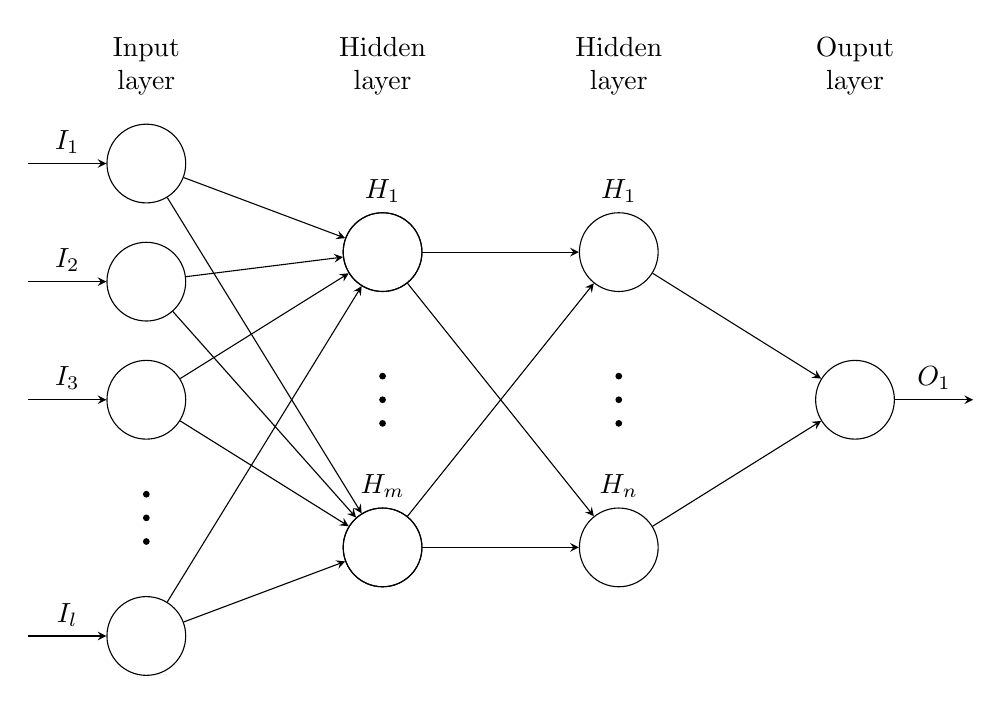
\begin{tikzpicture}[x=1.5cm, y=1.5cm, >=stealth]
					
					\foreach \m/\l [count=\y] in {1,2,3,missing,4}
					\node [every neuron/.try, neuron \m/.try] (input-\m) at (0,2.5-\y) {};
					
					\foreach \m [count=\y] in {1,missing,2}
					\node [every neuron/.try, neuron \m/.try ] (hidden1-\m) at (2,2-\y*1.25) {};
					
					\foreach \m [count=\y] in {1,missing,2}
					\node [every neuron/.try, neuron \m/.try ] (hidden1-\m) at (2,2-\y*1.25) {};
					
					\foreach \m [count=\y] in {1,missing,2}
					\node [every neuron/.try, neuron \m/.try ] (hidden2-\m) at (4,2-\y*1.25) {};
					
					\foreach \m [count=\y] in {1}
					\node [every neuron/.try, neuron \m/.try ] (output-\m) at (6,0.5-\y) {};
					
					\foreach \l [count=\i] in {1,2,3,l}
					\draw [<-] (input-\i) -- ++(-1,0)
					node [above, midway] {$I_\l$};
					
					\foreach \l [count=\i] in {1,m}
					\node [above] at (hidden1-\i.north) {$H_\l$};
					
					\foreach \l [count=\i] in {1,n}
					\node [above] at (hidden2-\i.north) {$H_\l$};
					
					\foreach \l [count=\i] in {1}
					\draw [->] (output-\i) -- ++(1,0)
					node [above, midway] {$O_\l$};
					
					\foreach \i in {1,...,4}
					\foreach \j in {1,...,2}
					\draw [->] (input-\i) -- (hidden1-\j);
					
					\foreach \i in {1,...,2}
					\foreach \j in {1,...,2}
					\draw [->] (hidden1-\i) -- (hidden2-\j);
					
					\foreach \i in {1,...,2}
					\foreach \j in {1}
					\draw [->] (hidden2-\i) -- (output-\j);
					
					\foreach \l [count=\x from 0] in {Input, Hidden, Hidden, Ouput}
					\node [align=center, above] at (\x*2,2) {\l \\ layer};
					\draw[fill=black](0,-1.3)circle(1pt);
					\draw[fill=black](0,-1.5)circle(1pt);
					\draw[fill=black](0,-1.7)circle(1pt);
					\draw[fill=black](2,-0.3)circle(1pt);
					\draw[fill=black](2,-0.5)circle(1pt);
					\draw[fill=black](2,-0.7)circle(1pt);
					\draw[fill=black](4,-0.3)circle(1pt);
					\draw[fill=black](4,-0.5)circle(1pt);
					\draw[fill=black](4,-0.7)circle(1pt);
					
				\end{tikzpicture}
		
		\caption{https://tex.stackexchange.com/questions/132444/diagram-of-an-artificial-neural-network}
		\label{fig: ownnet}
		\end{figure}
		
		Für den Einsatz am ALF ist die Erkennung anderer Objekte jedoch unerheblich. Somit gibt es unter anderem zwei Möglichkeiten diesen Sachverhalt zu lösen. Für den ersten Lösungsansatz wird das entsprechende KNN unverändert eingesetzt. Ein Sortieralgorithmus beschäftigt sich nach der Analyse des Bildes damit, nicht relevante Klassen auszusortieren. In Abbildung \ref{fig: ownnet} ist eine weitere Lösung dargestellt. Die Ausgabeschicht eines Netzes wird so verändert, dass lediglich ein Ausgangsneuron vorhanden ist. Dieser ist bekanntlich in der Lage auf eine Klasse trainiert zu werden. Die restlichen Klassen werden somit verworfen und das Neuron wird ausschließlich auf die Klasse \textit{Person} trainiert. Diese Vorgehensweise spart nicht nur die Einbindung eines Sortieralgorithmus, sondern auch Speicherplatz ein. Durch die Elimination der unbedeutsamen Neuronen werden folglich auch Parameter gelöscht, die gewissen Speicher einnehmen. Somit wird auch eine schnellere Rechenzeit erwartet. \\
		
		Zur Umsetzung des KNNs wird \textit{Tensorflow} der Firma \textit{Google} verwendet. \textit{Tensorflow} bietet neben der Möglichkeit des Trainings vortrainierter Netze, Lösungen zur Implementierung auf eingebetteten Systemen \cite{frameworks}. Diesbezüglich haben die Entwickler einen eigenen Framework namens \textit{Tensorflow Lite} ins Leben gerufen. Dieser Framework ist insbesondere für die Entwicklung mobiler Applikationen ausgelegt \cite{tflite}. \textit{Xus} Paper zeigt, dass \textit{Tensorflow} und \textit{Tensorflow Lite} die meistgenutzten Frameworks sind wenn es um mobile Applikationen geht. Weiterhin unterstützt der \textit{Tensorflow} die \textit{NVIDIA CUDA Deep Neural Network} (cuDNN) Bibliothek \cite{frameworks}. \textit{NVIDIA cuDNN} ist für Grafikprozessoren und der Arbeit mit künstlichen neuronalen Netzen optimiert \cite{frameworks}. Außerdem unterstützt \textit{Tensorflow} die Betriebssysteme \textit{Linux}, \textit{Mac OS X} und \textit{Windows} \cite{frameworks}. Somit kann der integrierte Computer des autonomen Logistikfahrzeugs als ausführende Instanz verwendet werden. Für Trainingsprozesse eignet sich in vielen Fällen ein Rechner mit einer leistungsstarken Grafikeinheit. Die Praxiserfahrung dieser Masterarbeit zeigte, dass eine Grafikkarte den Trainingsprozess um den Faktor 12 beschleunigt. Jedoch gibt es Anwendungsfälle, die durch die Verwendung der zentralen Recheneinheit des Computers beschleunigt werden \cite{cpugpu}. \\
		
		Als Datensatz für das Training der Netze wird der \textit{Common Objects in Context} (COCO) Datensatz der Firma \textit{Microsoft} verwendet. Dieser Datensatz enthält circa 330000 Bilder mit diversen alltäglichen Objekten \cite{coco, cocopaper}. Davon sind laut eigener Aussagen über 200000 Bilder mit sogenannten \textit{Annotations} oder auch \textit{Labels} (deutsch: Anmerkungen/Etiketten) versehen \cite{coco}. Die Daten sind in Trainings-, Evaluations- und Testdaten unterteilt. Letzteres ist jedoch nicht etikettiert und somit für dieses Masterarbeit nicht relevant. Die Trainingsdaten von dem \textit{COCO}-Datensatz aus dem Jahr 2017 stellt knapp 65000 etikettierte Bilder von Personen bereit. Circa 5000 Bilder sind im Evalutaionsdatensatz enthalten.\\
		
		Für den Lernprozess wird somit der Trainingsdatensatz in Trainings- und Testdaten unterteilt. So kann ein Teil der eigentlichen Trainingsdaten durch die vorhandenen Etiketten als Testdatensatz verwendet werden. Als zweiten Test wird ein eigener Datensatz erstellt. Hierbei werden 160 Bilder aus dem Einsatzumfeld des ALFs aufgenommen und etikettiert. In Kapitel \ref{ch: Verifikation} werden bereits besprochene Netze mit dem eigenen und dem \textit{COCO}-Datensatz evaluiert.
		
	\section{Konzept und Aufbau des Zustandsautomaten}
	\label{sec: Umsetzung der Statemachine}
	Bisher wurden für den Aufruf der Fahrfunktionen in \textit{ROS} ausführbare Dateien aufgerufen \cite{Bachelorarbeit}. Hierbei mussten der Benutzer darauf achten, diese Dateien nicht im geringen Zeitabstand und vor allem in der richtigen Reihenfolge aufzurufen. Zu jedem Anwendungsfall gehörten entsprechende Dateien. Ein hierarchischer Zustandsautomat nach Mealy unterbindet die Probleme, indem sich der Endzustand durch zuvor aufgerufene Zustände zusammensetzt. Der Aufruf verschiedner \textit{ROS}-Knoten in der korrekten Reihenfolge wird somit autark geregelt. Für die Steuerung des EAs wird die Spracherkennung aus der parallel laufenden Masterarbeit verwendet. Die Auswahl des Zustandsautomats wird im folgendem Kapitel näher ausgeführt.\\	
	
	\subsection{Auslegung des Zustandsautomats}
	Die Problematik der Steuerung über Sprache ist die Extraktion der eigentlichen Aussage eines Satzes. In der Masterarbeit von Hannes Dittmann werden aufgrund dessen Sprachbefehle kategorisiert \cite{Dittmann}. Die KI ist in der Lage verschiedene Sätze einer für den Roboter relevanten Kategorie zuzuordnen. Diese werden als Eingabeparameter für den EA genutzt. Weiterhin wird zwischen einer manuellen und einer autonomen Fahraufgabe unterschieden und als zweiten Parameter für den Zustandsautomaten genutzt. Anhand der technischen Fähigkeiten des Roboters wurden die Kategorienamen so gewählt, dass alle möglichen Handlungen abgedeckt sind. Der Zustandsautomat wurde so entworfen, dass er trotz der umfangreichen Fahrfunktionen des Roboters mit möglichst wenig Zuständen arbeitet. Außerdem deckt der Automat die Richtlinien nach Level 5 der in Kapitel \ref{ch: Einleitung} gezeigten Tabelle. Für die größtmögliche Effizienz hinsichtlich der Dimension und Funktionsweise des EAs wurde ein mathematisches Modell entworfen.\\
	
	\begin{equation}
	\vec{\epsilon}=\sum_{\epsilon_0}^{\epsilon_f} \left[ \begin{array}{r}
	k_0  \\
	k_{1}  \\
	...  \\
	k_8  \\
	\end{array}\right] \circ
	\left[ \begin{array}{r}
	g_0(\epsilon)  \\
	g_{1}(\epsilon)  \\
	...  \\
	g_8(z)  \\
	\end{array}\right]  \circ
	\left[ \begin{array}{r}
	1  \\
	1  \\
	m_{2}(\epsilon_f)  \\
	m_{3}(\epsilon_f)   \\
	1  \\
	m_{5}(\epsilon_f)  \\
	1   \\
	m_{7}(\epsilon_f)   \\
	m_8(\epsilon_f)  \\
	\end{array}\right]
	\text{ für }\epsilon_f\in[0;8] \text{ und }\epsilon_0=0 \vee 1
	\label{eq: statemachine}
	\end{equation}\\
	
		Anhand der Gleichungen \ref{eq: statemachine} und \ref{eq: Binärfunktion} wird der mathematische Hintergrund des EAs erläutert. Der hierarchische Zustandsautomat ermöglicht einen finalen, sich aufbauenden Zustand $\vec{\epsilon}$. Dieser wird anhand der in Gleichung \ref{eq: statemachine} dargestellten Summe berechnet. Beginnend vom Anfangszustand $\epsilon_0$ wird jeder mögliche $\epsilon$ bis zum finalen Zustand $\epsilon_f$ addiert. Bei der Addition geht es hauptsächlich darum, dem Anwendungsfall entsprechende \textit{ROS}-Knoten aufzurufen. Zu einem Zustand fest zugehörige Knotengruppen werden in Gleichung \ref{eq: statemachine} mit $k$ bezeichnet. Dessen Index deutet auf die Zugehörigkeit des Knotens zum jeweiligen Zustand. Hierbei werden die möglichen Endzustände wie in Abbildung \ref{fig: uml} nummeriert.\\
		
		Die Knotengruppe $k_0$ gehört zu dem Zustand \textit{Stop} und leitet den risikominalen Zustand ein. Dieser wird erreicht, indem alle \textit{ROS}-Knoten inklusive des des \textit{ROS}-Netzwerks heruntergefahren werden. So kann sichergestellt werden, dass keine Nachrichten an die Motorsteuergeräte der vier verbauten Motoren gesendet werden. Der Zustand \textit{Stop} kann nur verlassen werden, indem ein sicherer Wechsel in den Folgezustand \textit{Warten} durch den Benutzer zugesichert wird. Die Abfrage erfolgt sowohl über die Tastatur, als auch über Sprache. Alle folgenden Zustände enthalten der jeweiligen Anwendung entsprechende Knottengruppen. Eine Auflistung aller Zustände in im Anhang ... aufgeführt.\\ 
	
	\begin{equation}
	g(\epsilon)=\left\{\begin{array}{ll} 1 \text{ für } \epsilon=n \\
	0 \text{ für }\epsilon\neq n\end{array}\right. 
	\label{eq: Binärfunktion}
	\end{equation}\\
		
		Gleichung \ref{eq: Binärfunktion} zeigt die verwendete Binärfunktion $g(\epsilon)$. Je nach Iterationsschritt de- und aktiviert die Funktion $g(\epsilon)$ rein binär die korrekte Zeile in Gleichung \ref{eq: statemachine}. Nicht aktive Zustände werden mit 0 multipliziert sowie aktive mit einer einfachen Verstärkung beaufschlagt. \\
		
		Die ebenfalls binären Vektorelemente $m_n(\epsilon_f)$ sind mathematisch von der Zusammensetzung des Endzustands abhängig. Dieser Sachverhalt wird beispielsweise mithilfe der manuellen Fahrfunktion erklärt. Diese wird automatisiert mit einer statischen Karte gestartet, in der sich der Roboter durch einen Partikelfilter selbst findet. Hat der Benutzer jedoch zuvor eine Lokalisierung mithilfe der \textit{SLAM}-Methode gefordert, kann dieselbe Fahraufgabe mit einer sich aufbauenden Karte vollzogen werden. Widerrum schließen sich diverse Zustände gegenseitig aus. Eine bestimmte Zielpose ist von dem Ursprung einer statischen Karte abhängig. Diese ist beim \textit{SLAM}-Algorithmus jeodch nicht vorhanden. So kann folglich kein Ziel angefahren werden, wenn zuvor die Lokalisierung mithilfe von \textit{SLAM} abgeschlossen wurde.\\
		
		\begin{figure}[H]
			\centering
			\begin{minipage}[b]{0.4\textwidth}
				\begin{equation}
					m_2(\epsilon_f)=\left\{\begin{array}{ll} 1 \text{ für } \epsilon_f=2,7 \\
					0 \text{ für }\epsilon_f\neq 2,7\end{array}\right. 
					\label{eq: m2}
				\end{equation}\\
			\end{minipage}
			\hfill
			\begin{minipage}[b]{0.55\textwidth}
				\begin{equation}
					m_3(\epsilon_f)=\left\{\begin{array}{ll} 1 \text{ für } \epsilon_f\neq2,7 \wedge m_2(\epsilon_f) = 0 \\
					0 \text{ für }\epsilon_f= 2,7\end{array}\right.
					\label{eq: m3}
				\end{equation}\\
			\end{minipage}
		\end{figure}
		
		Nur einer der Vektorelemente $m_2(\epsilon_f)$ und $m_3(\epsilon_f)$ kann aktiv sein. Der Modus entspricht auch hier dem Index und sagt aus, ob die Fahraufgabe mit einer statischen oder einer sich aufbauenden Karte bearbeitet werden soll. Hierfür gelten die bereits angesprochenen Restriktionen. Die drei fahrfähigen Endzustände \textit{Manuell}, \textit{Erkunden} und \textit{Ziel} werden durch $m_5$, $m_7$ und $m_8$ aktiviert. Der Zustandsautomat besitzt die Fähigkeit diverse Zwischenzustände, als temporäre Endzustände $\epsilon_f$ auszuführen. Somit kann sich das ALF beispielsweise im Modus \textit{Statische Karte} $\epsilon_f=3$ ohne eine bestimmte Fahraufgabe selbst lokalisieren. In einem weiteren Schritt ist es dem Benutzer erlaubt vollständige und fahrfähige Endzustände auszuwählen wie zum Beispiel den Modus \textit{Ziel} $\epsilon_f=8$.\\
		
		
				\begin{equation}
					m_5(\epsilon_f)=\left\{\begin{array}{ll} 1 \text{ für } \epsilon_f=5 \\
						0 \text{ für }\epsilon_f\neq 5\end{array}\right. 
					\label{eq: m5}
				\end{equation}\\
			
		Auch bei den genannten, fahrfähigen Endzuständen gibt es diverse Einschränkungen. So kann der manuelle Fahrmodus nur ausgewählt werden, wenn er als Endzustand $\epsilon_f$ definiert wurde. Die entsprechende Logik ist in Gleichung \ref{eq: m5} gezeigt.\\
		
				\begin{equation}
					m_7(\epsilon_f)=\left\{\begin{array}{ll} 1 \text{ für } \epsilon_f=7 \wedge m_2(\epsilon_f)=1 \wedge m_5(\epsilon_f)=0 \\
						0 \text{ für }\epsilon_f\neq 7\end{array}\right.
					\label{eq: m7}
				\end{equation}\\
				
		Gleichung \ref{eq: m7} stellt die Restriktionen des Zustands \textit{Erkunden} dar. Wenn der Modus als Endzustand gewählt wurde, die Lokalisierung ausschließlich durch die \textit{SLAM}-Methode realisiert wird und zuvor kein fahrfähiger Endzustand aktiviert wurde, darf der Zustand \textit{Erkunden} in Kraft treten. Für den Zustand \textit{Ziel} gilt grundlegend diesselbe Logik für die Aktivierung. Jedoch verlangt der Fahrmodus eine statische Karte. In Gleichung \ref{eq: m8} sind die Abhängigkeiten genauer verdeutlicht.\\
		
		
				\begin{equation}
					m_8(\epsilon_f)=\left\{\begin{array}{ll} 1 \text{ für } \epsilon_f=8 \wedge m_3(\epsilon_f)=1 \wedge m_5(\epsilon_f)=0 \wedge m_7(z_f)=0 \\
						0 \text{ für }\epsilon_f\neq 8\end{array}\right.
					\label{eq: m8}
				\end{equation}\\
		
		Für eine übersichtliche Darstellung eines Zustandsautomats eignet sich ein \textit{Unified Modeling Language} (UML) Diagramm. Das zum entworfenen Zustandsautomaten entsprechende UML-Diagramm ist in Abbildung \ref{fig: uml} gezeigt. Zustände sind als Boxen mit Abrundungen dargestellt und durch den Namen sowie den dazugehörigegen Index kennzeichnet. Pfeile stehen für Transitionen zwischen den Zuständen. Je nach Hierarchieebene legen schwarze Punkte den Startpunkt fest, der durchlaufen werden muss. 
		
	
	
	
	\begin{figure}[H]
	\centering

\begin{tikzpicture}[round/.style={rounded corners=1.5mm,minimum width=3cm,inner sep=2mm,above right,draw,align=left}]

\node[round] (stop) at (1,10) {Stop 0};
\node[round] (wait) at (1,8) {Warten 1};
\node[round] (localization) at (3.5,6) {Statische Karte 3};
\node[round] (slam) at (-1.5,6) {SLAM 2};
\node[] (autonomname) at (5,2) {Autonom 6};
\node[round] (explore) at (6,0) {Ziel 8};
\node[round,align=center] (goal) at (1,0) {Erkunden 7};
\node[round,above,fit=(explore)(goal)(autonomname)] (autonom) {};
\node[round,align=center] (manual) at (-4,0) {Manuell 5};
\node[] (drivename) at (2.5,4) {Fahren 4};
\node[round,fit=(manual)(autonom)(drivename)] (drive) {};

\draw[-latex] ($(stop.north) + (-0,0.5)$) coordinate (temp) to (stop);
\fill (temp) circle (0.1);
\draw[-latex]  (stop) to (wait);
\draw[-latex,bend left]  (wait.333) to (localization.north);
\draw[-latex,bend right]  (wait.207) to (slam.north);
\draw[-latex,bend left]  (slam.south) to (drive.north);
\draw[-latex,bend right]  (localization.south) to (drive.north);
\draw[-latex,bend right] ($(autonom.north) + (-2.5,1)$) coordinate (temp2) to (manual.north);
\draw[-latex,bend left] ($(autonom.north) + (-2.5,1)$) coordinate (temp2) to (autonom.110);
\fill (temp2) circle (0.1);
\draw[-latex,bend right] ($(goal.north) + (2.5,0.8)$) coordinate (temp3) to (goal.north east);
\draw[-latex,bend left] ($(goal.north) + (2.5,0.8)$) coordinate (temp3) to (explore.north west);
\fill (temp3) circle (0.1);
%\draw[-latex, bend left] ($(neutral.north east) + (-0.5,0.3)$) coordinate (temp3) to (neutral);
%\fill (temp3) circle (0.1);
%\draw[-latex, bend left] (left) to (right);
%\draw[-latex, bend left] (right) to (left); 
%\draw[-latex, bend left] (left) to (neutral);
%\draw[-latex, bend left] (neutral) to (right);
%\draw[-latex, bend left] (neutral) to (left);
%\draw[-latex, bend left] (right) to (neutral);
%
%\draw[-latex, bend left] (pause) to (running);
%\draw[-latex, bend left] (pause) to[in=-135,out=-90] (ident);
%\draw[-latex, bend left] (pause) to (observe);
%\draw[-latex, bend left] (observe) to (origin);
%%\draw[-latex, bend left] (origin) to (origin);
%\draw[-latex, bend left] (origin) to (pause);
%\draw[-latex, bend left] (running) to (origin);
%\draw[-latex, bend left] (ident) to[out=-60,in=-90] (origin);
%\draw[-latex, bend left] (rotLeft) to (rotRight);
%\draw[-latex, bend left] (rotRight) to (rotLeft);
\end{tikzpicture}
\caption{Konzept eines hierarchischen Zustandsautomaten in Form eines UML-Diagramms. Zustände sind als Boxen mit Abrundungen dargstellt. Ineinander verschachtelte Zustände erben Funktionen von dem jeweils größeren Zustand. Pfeile deuten mögliche Transitionen an. Startzustände werden durch schwarze Punkte gezeigt. Adaptiert aus \cite{texex}.}
\label{fig: uml}
\end{figure} 
	
	\section{Funktionsweise des Gesamtsystems}
	\label{sec: Funktionsweise des Gesamtsystems}
		
	Der Kern dieser Arbeit ist die Personenerkennung im praktischen Kontext des im Kapitel \ref{ch: Einleitung} beschriebenen autonomen Logistikfahrzeugs. In Abschnitt \ref{sec: Anforderungserhebung} wurden bereits alle Schnittstellen zu verbauten Hardware- und Softwarekomponenten präsentiert. Das vollständige System der Personenerkennung ist im Folgenden erklärt.\\
	
	Wie bereits in dem Kapitel \ref{ch: Einleitung} dieser Masterarbeit beschrieben, wird die Personenerkennung am ALF mithilfe der Bildinformationen von zwei \textit{Kinect}-Kameras betrieben. Als Programmiersprache wird im Zuge dieser Masterarbeit \textit{Python} verwendet. Mit Softwarepaketen wie beispielsweise \textit{OpenCV} oder \textins{Pillow} bietet \textit{Python} ein großes Spektrum an Softwarelösungen für die Bildverarbeitung \cite{opencv}\cite{pillow}. Viele bekannte Frameworks wie \textit{Tensorflow} oder \textit{Keras} unterstützen \textit{Python}.\\
	
	Wie auch im Projekt der Bachelorarbeit, liefert das integrierte \textit{ROS}-Netzwerk die Bildinformation der Kameras. Die Schnittstelle zwischen \textit{ROS} und \textit{Python} bietet die Möglichkeit eingehende Bilder sowohl parallel, als auch seriell zu bearbeiten. Jedoch ist zu beachten, dass die Recheneinheit eines Computers durchaus mit der Bildverarbeitung eines Bildes mit bis zu über 50 \percent\text{ } Rechenkapazität belastet sein kann. Demzufolge ist auf einem eingebettetem System eine deutlich höhere Belastung zu erwarten. Aufgrunddessen wird bei der Bildverarbeitung der Personenerkennung auf eine serielle Bearbeitung gesetzt. Zu Beginn arbeitet das System in einem reduzierten Modus. Hierbei werden Pausen mit der gewünschten Dauer zwischen Bildverarbeitungsprozessen eingelegt bis ein relevantes Bild erkannt wird. Erst dann arbeitet die Personenerkennung mit der maximalen Geschwindigkeit. Der reduzierte Modus erspart weitere Rechenkapazität des Computers für parallel laufende Prozesse. Als relevant werden Bilder eingestuft, die eine Person enthalten.\\
	

	In Abbildung \ref{fig: Personenerkennung} wird der Ablauf der Personenerkennung in Form eines Programmablaufplans dargestellt. Die Darstellung zeigt die Funktionsweise des Programms ab dem Zeitpunkt, an dem eine Person von einer Kamera detektiert wird. Zu Beginn der Analyse gelangt jedes Bild in das verwendete künstliche neuronale Netz. Je nach Anzahl der erkannten Person werden korrespondierende Begrenzungsrahmen ausgegeben, die die Position des Interessensbereichs im Bild beschreiben. Dieser Vorgang ist beispielhaft in Darstellung \ref{fig: bbox} präsentiert. Die dort abgebildeten Personen werden in diesem Fall von einem roten Begrenzungsrahmen umrandet. Wird keine Person erkannt, verfällt das Programm wieder in den bereits beschriebenen, reduzierten Modus. Die extrahierten Begrenzungsrahmen gelten im Falle einer Personendetektion als Interessensbereich der Gesichtserkennung.\\
	
		\newpage
	\begin{figure}[H]
		\centering
		\begin{tikzpicture}[node distance = 1.2cm, auto]
			
			% Place nodes
			\node [papStart] (Start1){Start};
			\node [papProcess, below of = Start1] (pro1){Prozess};
			\node [papDecision, below of = pro1, yshift= -9mm,label={[align=left,anchor=west,shift={(1.2,-0.3)}]\footnotesize\textit{Menschen im Bild?}}](dec1){Entscheidung};
			\node [papProcess, right of = dec1,xshift=25mm](pro3){Prozess};
			\node [papDecision, below of = pro3, yshift= -9mm](dec2){Entscheidung};
			\node [papProcess, below of = dec2, yshift= -9mm](pro4){Prozess};
			\node [papDecision, below of = pro4, yshift= -9mm,label={[align=left,anchor=west,shift={(1.2,-0.3)}]\footnotesize\textit{Gesicht bekannt?}}](dec3){Entscheidung};
			\node [papDecision, below of = dec3, yshift= -18mm,label={[align=left,anchor=west,shift={(1.2,-0.3)}]\footnotesize\textit{\makecell[l]{Registrierungs-\\prozess\\einleiten?}}}](dec4){Entscheidung};
			%\node [papData, right of = dec3, xshift= 25mm,label={[shift={(5,-0.6)}]\footnotesize\textit{Gesicht bekannt?}}](dat1){I/O};		
			\node [papProcess, below of = dec4,yshift= -9mm](pro6){Prozess};
			\node [papProcess, below of = pro6](pro5){Prozess};
			\node [papEnd, below of = pro5,xshift=-37mm] (End) {Ende};
			
			\node[right of = pro1,xshift=0.5cm,align=left,anchor=west] (P1) {\footnotesize\textit{\makecell[l]{Personendetektion\\durch KNN}}};
			\node[right of = pro3,xshift=0.5cm,align=left,anchor=west] (P2) {\footnotesize\textit{\makecell[l]{Gesichtsdetektion\\durch KNN}}};
			\node[right of = dec2,xshift=0.5cm,align=left,anchor=west] (D2) {\footnotesize\textit{\makecell[l]{Gesicht im\\Interessenbereich?}}};
			\node[right of = pro4,xshift=0.5cm,align=left,anchor=west] (P3) {\footnotesize\textit{\makecell[l]{Merkmalsextraktion\\des Gesichts}}};
			\node[right of = pro6,xshift=0.5cm,align=left,anchor=west] (P1) {\footnotesize\textit{\makecell[l]{Person\\registrieren}}};
			\node[right of = pro5,xshift=0.5cm,align=left,anchor=west] (P1) {\footnotesize\textit{\makecell[l]{Person\\aktualisieren}}};
			
			% Place joins
			\coordinate [below of = dec1, yshift= -9mm] (join1);
			\coordinate [right of = dec3,xshift=25mm] (join2);
			\coordinate [left of = dec4, xshift= -25mm] (join3);
			\coordinate [right of = pro5,xshift=25mm] (join4);
			\coordinate [left of = pro5,xshift=-25mm] (join5);
			
			% Draw edges
			\path [papLine] (Start1) -- (pro1);
			\path [papLine] (pro1) -- (dec1);
			\path [papLine] (dec1) -- node [above] {\papYes} (pro3);
			\draw (dec1) -- node [left] {\papNo} (join1);
			\path [papLine] (pro3) -- (dec2);
			%	\path [papLine] (dec2) -- node [above] {\papYes} (pro4)
			\draw (dec2) -- node [above] {\papNo} (join1);
			\path [papLine] (dec3) -- node [left] {\papNo} (dec4);
			\draw (dec3) -- node [above] {\papYes} (join2);
			\path [papLine] (join1) -- (End);
			\draw (dec4) -- node [above] {\papNo} (join3);
			\draw (join2) -- (join4);
			\path [papLine] (join4) -- (pro5);
			\draw (pro5) -- (join5);
			\path [papLine] (dec4) -- node [left] {\papYes} (pro6);
			\path [papLine] (pro6) -- (pro5);
			\path [papLine] (dec2) -- node [left] {\papYes} (pro4);
			\path [papLine] (pro4) -- (dec3);
			
		\end{tikzpicture}
		\caption{Prozessablaufplan der Personenerkennung. Der Start sowie das Ende des Programms sind als Boxen mit Abrundungen dargestellt. Rechtecke zeigen Prozesse und Parallelogramme deuten eine Entscheidung im Programmablauf an. Die Flussrichtung der entsprechenden Informationen werden durch Pfeile präsentiert. Adaptiert aus \cite{texwelt}.}
		\label{fig: Personenerkennung}
	\end{figure}

	\begin{figure}[H]
		\centering
		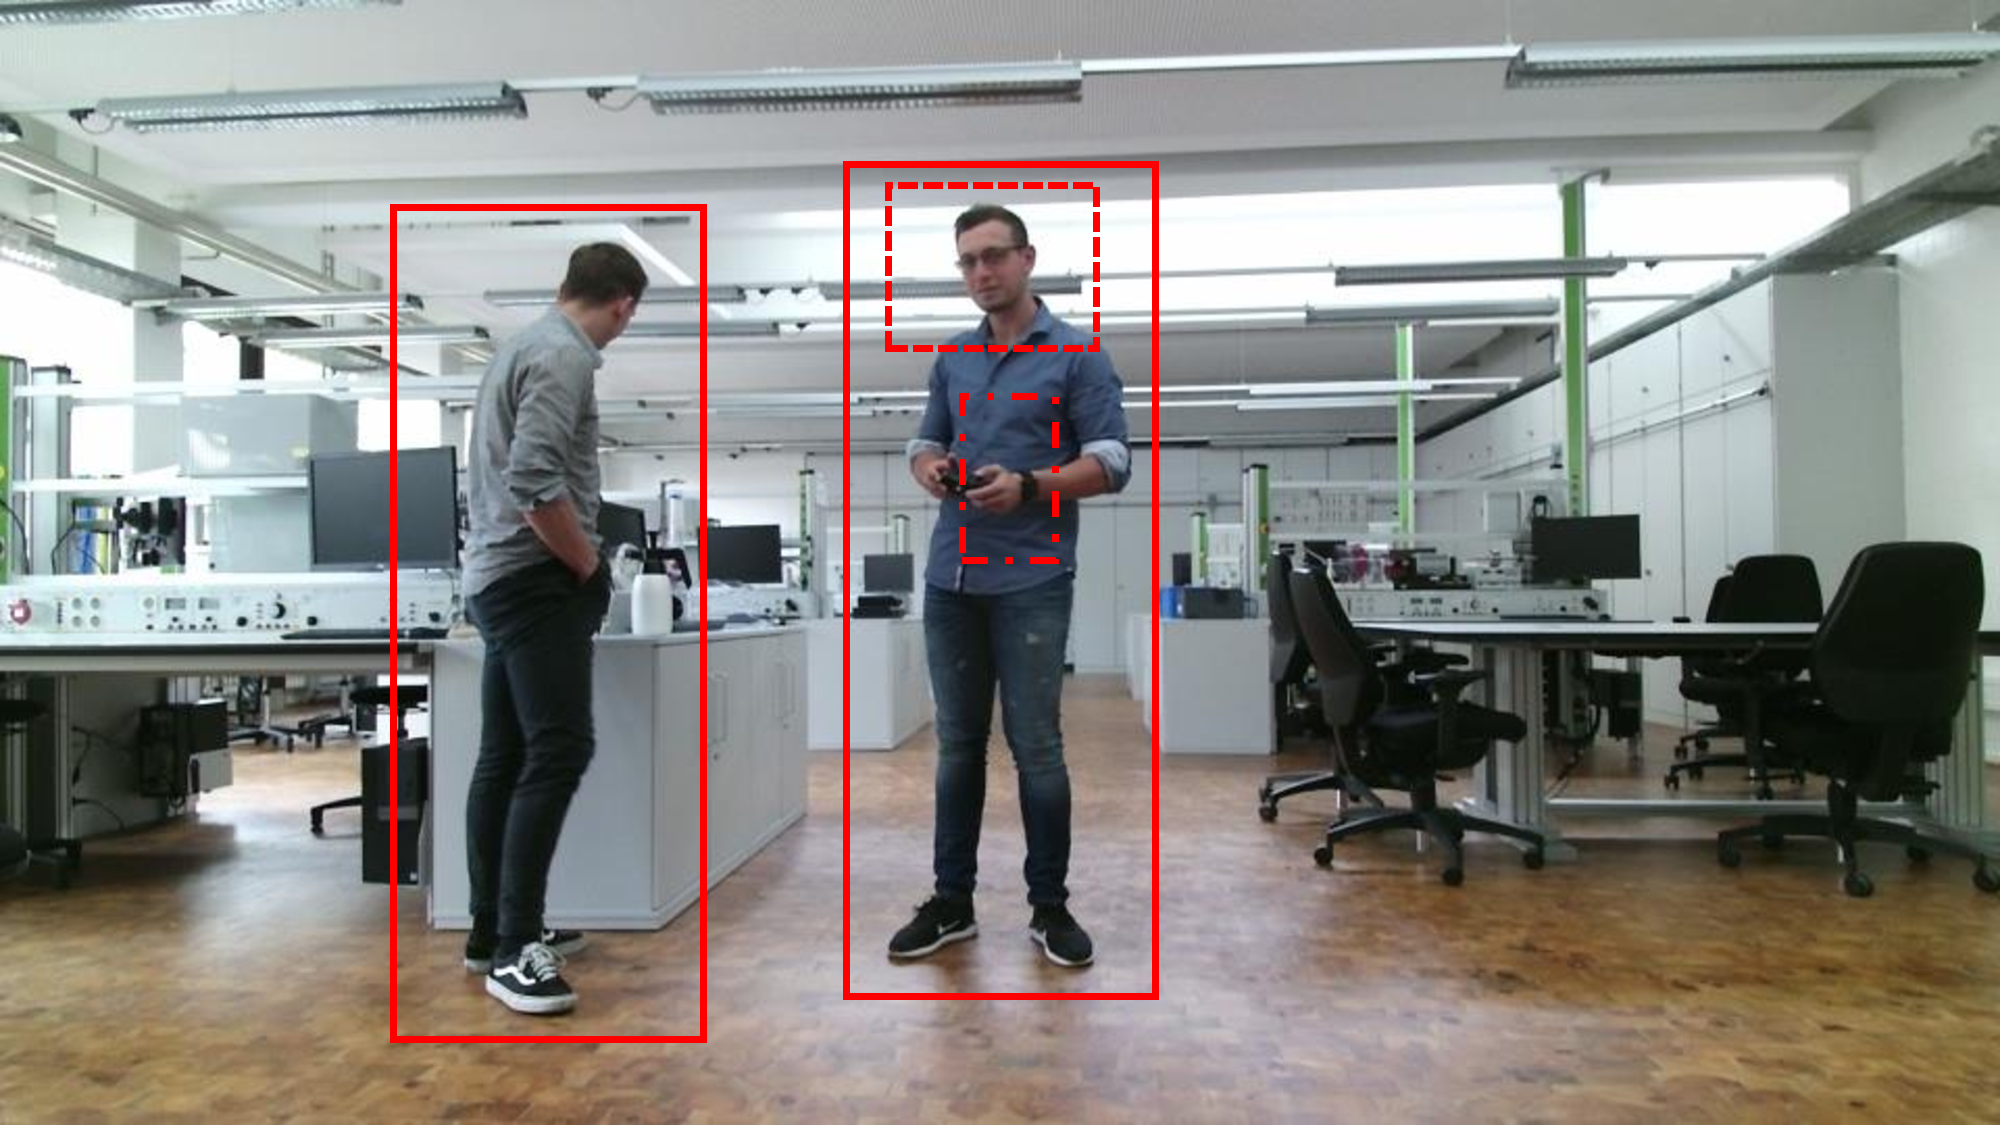
\includegraphics[width=1\textwidth]{Bilder/person.pdf}
		\caption{Konzept eines Fallbeispiels der Personenerkennung. Zu sehen sind zwei Personen im Labor für Antriebstechnik der Hochschule Bochum. Rote Rechtecke zeigen den Interessensbereich der Personendetektion. Der Begrenzungsrahmen der Gesichtsdetektion ist gestrichelt dargestellt. Das als Strichpunkt präsentierte Rechteck deutet den Bereich der Distanzmessung an.}
		\label{fig: bbox}
	\end{figure}
	
	Das Pythonpaket \textit{face-recognition} wird in diesem Projekt für die Gesichterkennung verwendet. Prinzipiell arbeitet das Paket in drei Schritten. Die in Kapitel \ref{subsec: Objekterkennung durch alternative Verfahren} erklärte \textit{HoG}-Methode wird zur Extraktion des Begrenzungsrahmens des jeweiligen Gesichts angewendet \cite{facerecarticle}. Damit eine Person nicht unbedingt gerade in das entsprechende Aufnahmegerät schauen muss, werden durch die Software sogenannte Landmarken auf dem Gesicht verteilt \cite{facerecarticle}. Diese werden zur Rotation des Gesichts im Bild verwendet \cite{facerecarticle}. Das bearbeitete Bild des Gesichts wird mit einem neuronalen Netz analysiert, dass von den Entwicklern von \textit{OpenFace} bereitsgestellt wird \cite{facerecarticle}. Entwickler \textit{Adam Geitgey} gibt für das im Paket verwendete Netz eine Genauigkeit von 99,38$\percent$ an \cite{facerecognition}. Hinsichtlich der in Kapitel \ref{ch: Grundlagen} besprochenen, möglichen Nutzungsszenarien der Personenerkennung, ist eine hohe Genauigkeit notwendig. Nach eigener Recherche besitzen die von \textit{OpenFace} bereitgestellten, neuronalen Netze zwischen 3,7 - 7,4 Millionen Parameter \cite{openface}. Die Größenordnung ähnelt folglich die einer herkömmlichen \textit{MobileNet}-Architektur. Außerdem bietet das \textit{face-recognition} Paket eine Funktion zum Vergleichen und Unterscheiden von Gesichtsmerkmalen. Aufgrund der Genauigkeit und der verwendeten Netze, wird das das \textit{face-recognition} Paket in dieser Masterarbeit für die Gesichtserkennung eingesetzt.\\
	
	Im Zuge der Gesichtserkennung kann davon ausgegangen werden, dass sich das Gesicht einer Person im oberen Teil des extrahierten Begrenzungsrahmens befindet. Dafür wird der Interessensbereich verkleinert. Somit muss die Gesichtserkennung nicht den vollständigen Interessensbereich durchsuchen und es wird weitere Rechenkapazität eingespart. Sollte sich kein Gesicht im relevanten Bereich befinden, wird davon ausgegangen, dass die Person stark von der Kamera abgewandt ist. Somit ist keine eindeutige Identifikation möglich und es erfolgt ein Neustart des Programms.\\
	
	Detektiert das Netz jedoch ein Gesicht wird eine Merkmalsextraktion durchgeführt. Im Anschluss werden die extrahierten Merkmale mit den, der bereits abgespeicherten Gesichter verglichen. Wird kein übereinstimmendes Gesicht gefunden, leitet das System ein Registrierungsprozess ein. Je nach Einstellung wird ein Gesicht registriert, wenn es entsprechend oft hintereinander erkannt worden ist. Im Falle der Erkennung eines bekannten Gesichts werden Eiegenschaften der erkannten Person, wie zum Beispiel die Gesichtsmerkmale oder die Position in der aktuellen Karte aktualisiert. \\ 
	
	  

	

		
	
		
		
				   		

